\chapter{Confronto tra i linguaggi}
\subsubsection{Sintassi}
Objective-C, in quanto lunguaggio basato su C, ha introdotto nuove parole chiave per differenziare i nuovi tipi da quelli C, utilizzando il simbolo @. Swift, in quanto linguaggio indipendente non applica alcuna distinzione.\\
Swift elimina inoltre le convenzioni utilizzate nei linguaggi di programmazione con qualche decade sulle spalle e non solo: non è necessario utilizzare il punto e virgola per terminare un blocco di codice, non sono necessarie le parentesi per le espressioni condizionali negli statement if/else.\\
Una differenza sostanziale rispetto ad Objective-C sono le chiamate di funzione, che utilizzano la sintassi puntuale invece di quella con le parentesi quadre. Gli argomenti di funzione inoltre utilizzano la più comune virgola rispetto alle parentesi quadre innestate
\subsubsection{Manutenzione del codice sorgente}
Swift è più semplice da mantenere\\
Objective-C non può evolvere senza attendere l'evoluzione del linguaggio C sottostante; quest'ultimo richiede al programmatore il mantenimento di due files separati per migliorare il tempo di compilazione e l'efficienza di esecuzione, problema che si ripercuote su Obj-C.\\
In Swift questo problema non si presenta e il compilatore riconosce dipendenze automaticamente e performa build incrementali, il tutto utilizzando un singolo file.
\subsubsection{Tooling}
I meccanismi ausiliari di aiuto alla programmazione, quali evidenziazione della sintassi ed i suggerimenti di Swift non sono ancora alla pari di quelli Objective-C, fatto che si rende evidente confrontando due files scritti nei due linguaggi in XCode. Inoltre, gli strumenti di refactoring non sono ancora disponibili per Swift.
\subsubsection{Runtime}
Il runtime di Objective-C è generalmente più robusto e permette meccanismi quali reflection e deep introspection di oggetti e tipi, che al momento non sono disponibili in Swift
\subsubsection{Sicurezza} 
Un aspetto interessante di Objective-C è il comportamento dei puntatori (in particolare quelli nil). In questo linguaggio non accade nulla se si chiama un metodo con una variabile puntatore non inizializzata: questa linea di codice viene considerata una non-operazione (no-op). Questo comportamento può avere effetti impredicibili, poichè può provocare effetti collaterali sull'esecuzione del programma.\\
I tipi optional di Swift invece offrono la possibilità di avere una gestione chiara del tipo nil, e genera errori a tempo di compilazione. Questo permette di creare un ciclo di feedback molto ristretto per lo sviluppatore e fa si che si scriva codice con attenzione a questo tipo di problema.\\
Tipicamente, in Objective-C, se un valore viene ritornato da una funzione è compito dello sviluppatore documentare il comportamento del puntatore ritornato (utilizzando commenti e convenzioni di nome); questo non accade in Swift in quanto il tipo optional permette a priori di capire se il valore esiste o se ha la possibilità di essere nil.\\ Per offrire un comportamento predicibile Swift genera un crash a runtime se una variabile nil di tipo optional è utilizzata.\\
\subsubsection{Tempi di scrittura del codice}
Come già analizzato, il tempo di scrittura di una classe in Swift è notevolmente minore grazie al singolo file necessario per la dichiarazione e definizione della stessa.\\Altre caratteristiche di Swift che permettono di risparmiare tempi di scrittura sono la concatenazione di stringhe tramite l'operatore + (operazione non possibile in Objective-C), oltre alla possibilità di interpolare stringhe senza dover utilizzare sintassi quali \%s, \%d, \%@). Il sistema di tipi in Swift inoltre riduce la complessità degli statements grazie alla type inference, ovvero la capacità del compilatore di capire il tipo degli oggetti senza la necessità di esplicitarlo nel codice.
\subsubsection{Namespaces nei progetti open source}
Uno dei problemi di Objective-C è la mancanza di supporto formale ai namespaces, soluzione utilizzata per evitare collision di nome nei files.\\Quando ciò accade in questo linguaggio si ha un errore a livello di linking.\\Alcune convenzioni sono state utilizzate, come per esempio prefissi a due o tre lettere per differenziare il codice scritto da un programmatore rispetto ad un altro, per esempio nei progetti condivisi su github, contenenti frameworks.\\
Swift supporta i namespaces permettendo quindi l'esistenza dello stesso file in progetti multipli senza causare un errore nel building, poichè sono basati sul target che contiene il file; questo significa che il programmatore può differenziare le classi o valori utilizzando l'identificatore del namespace.\\
In termini pratici ciò significa che nella collaborazione in progetti open source è possibile creare files con lo stesso nome evitando comunque collisioni ed errori in compilazione.\\
\subsubsection{Librerie dinamiche}
Un aspetto che ha suscitato poco clamore ma che può apportare benefici notevoli nel lungo periodo sono le librerie dinamiche di Swift: queste sono pezzi di codice eseguibile che possono essere collegati da un'applicazione. Questa caratteristica permette alle applicazioni già pubblicate di avere aggiornamenti delle librerie col susseguirsi delle versioni del linguaggio.\\Lo sviluppatore invia sullo store l'applicazione insieme alle librerie, digitalmente firmate per assicurarne l'integrità, questo significa che Swift può evolvere più velocemente di iOS stesso, poichè gli aggiornamenti della libreria possono essere inclusi direttamente in un aggiornamento dell'applicazione.\\
\subsubsection{Open Sourcing}
Swift è stato reso open source nel Dicembre del 2015, permettendo agli sviluppatori di influenzare il futuro del linguaggio; questo ha già portato a notevoli cambiamenti nella struttura dello stesso nel passaggio dalla versione 2.3 alla 3.0  
\section{Gestione della memoria}
Esistono due modalità di gestione della memoria:\\
\\-MMR (Manual retain-release), dove lo sviluppatore gestisce esplicitamente la memoria, tenendo traccia degli oggetti instanziati. E' implementato tramite un modello chiamato Reference Counting, fornito dalla classe NSObject in congiunzione all'ambiente di runtime; è il metodo più obsoleto e più dispendioso in termini di tempo di sviluppo in quanto è un approccio prettamente manuale.\\
\\-ARC (Automatic reference counting), che utilizza lo stesso sistema di tracciamento degli oggetti di MMR, ma aggiunge automaticamente chiamate ai metodi di gestione della memoria a tempo di compilazione. Questo sistema permette di assicurare che gli oggetti abbiano vita il tempo necessario per il loro utilizzo e non oltre, poichè il compilatore genera in automatico anche i metodi di dealloc appropriati.\\E' l'approccio moderno e più utilizzato della gestione della memoria in Objective-C e Swift.
\begin{figure}[H]
      \centering
      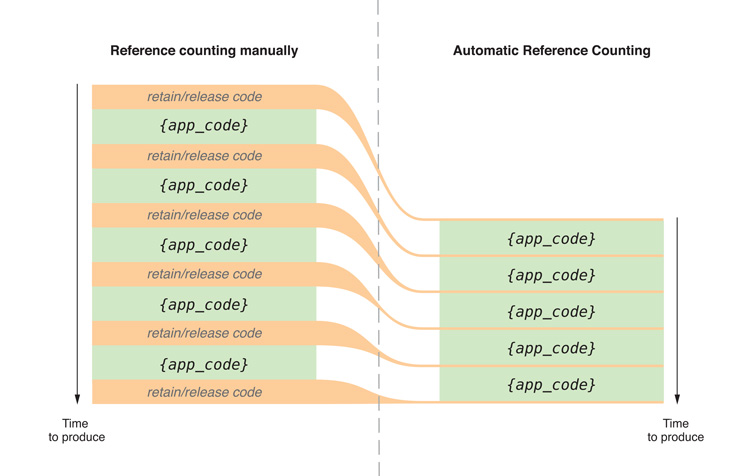
\includegraphics[scale=0.40]{immagini/ARC.jpg}
            \vspace{0.8cm}
            \caption{\textit{Confronto tra MMC ed ARC relativo al tempo di creazione dei cicli di retain-release degli oggetti}}
    \end{figure}
Il comportamento di ARC è però differente tra i due linguaggi:\\
In Swift il supporto è completo rispetto ai percorsi di codice procedurali ed object oriented; Objective-C invece supporta ARC solamente nell'utilizzo delle API Cocoa ed il codice object-oriented, questo significa che sarà ancora compito del programmatore gestire la memoria quando vengono utilizzate API come Core Graphics e altre di basso livello disponibili in iOS, creando il rischio di memory leaks.
\subsubsection{Performance}



